\chapter{Analysis and Specifications}
\label{chap:Analysis_and_Specifications}

\section*{Introduction}
This chapter is dedicated to delineating the detailed specifications and requirements of the proposed LegalTech platform. A rigorous analysis is essential to ensure the system architecture aligns with both the overarching project objectives and the specific expectations of end-users. In the subsequent sections, we categorize these specifications into functional requirements, detailing the explicit capabilities the system must exhibit; non-functional requirements, outlining the performance and operational standards; and system constraints, which establish the developmental, financial, and technological boundaries.

\newpage

\section{Functional Requirements}
This section enumerates the functional requirements foundational to the platform's architecture. These represent the core features and behaviors the system must support to facilitate a robust, AI-powered legal application.

\subsection{User Interface (UI)}
\begin{itemize}
    \item \textbf{Landing Page:} The platform shall provide an intuitive, user-centric landing page that clearly articulates the application's core concept, value proposition, and primary functionalities.
    \item \textbf{Account Creation \& Login:} Users must be empowered to create an account and authenticate securely utilizing multiple Identity Providers (IdPs), including Email/Password, Google, Facebook, and Apple ID.
    \item \textbf{AI Chat Interface:} A dedicated conversational interface must be provisioned, allowing users to interact directly with the Large Language Model (LLM) augmented by the RAG pipeline.
    \item \textbf{File Upload \& Management:} Users must be able to upload personal documents directly into the chat interface. Additionally, they require a persistent, personal cloud repository to store documents and import them into active chat sessions on demand.
    \item \textbf{Document Generation:} The platform shall enable users to draft formal legal documents manually using \LaTeX\ via direct code input within an integrated IDE.
    \item \textbf{AI-Assisted Drafting:} Users shall have the ability to prompt the AI assistant to autonomously draft, format, or modify legal documents utilizing a centralized registry of pre-existing templates.
\end{itemize}

\subsection{Large Language Model (LLM) Integration}
\begin{itemize}
    \item \textbf{Model Selection:} The platform must seamlessly integrate a highly capable, state-of-the-art LLM optimized for complex legal reasoning and multilingual comprehension.
    \item \textbf{Context Memory:} The conversational agent must retain conversational context, effectively remembering previous prompts and uploaded documents within a contiguous session.
    \item \textbf{Role Prompting:} The LLM must be strictly governed by engineered system prompts, enforcing rigorous rules and constraints to ensure it consistently operates within its designated persona as a Moroccan legal assistant.
\end{itemize}

\subsection{Data Retrieval (RAG System)}
\begin{itemize}
    \item \textbf{RAG Architecture:} A Retrieval-Augmented Generation (RAG) paradigm shall be implemented to synthesize LLM-generated responses with highly relevant, empirically factual data extracted from a curated document corpus.
    \item \textbf{Standardized Retrieval Mechanism:} The system shall leverage specialized Vector Stores (ChromaDB) to facilitate rapid, efficient, and semantically precise searches based on user queries.
\end{itemize}

\subsection{Authentication and Authorization}
\begin{itemize}
    \item \textbf{Multi-Provider Auth:} The system must implement robust, enterprise-grade authentication by integrating third-party OAuth providers via Clerk.
    \item \textbf{Admin Dashboard:} A secure, restricted-access dashboard must be exclusively available to platform administrators for user governance and systemic monitoring.
\end{itemize}

\subsection{System Monitoring and Reporting}
\begin{itemize}
    \item \textbf{Smart Logging System:} An automated, highly structured telemetry mechanism must be implemented. To optimize disk storage, logs shall be compressed into \texttt{.gz} archives daily and subjected to a 30-day rolling deletion policy.
    \item \textbf{Automated API Retry Mechanism:} To minimize error rates and ensure high availability, backend controllers must autonomously retry transiently failed API requests prior to propagating errors to the client.
\end{itemize}

\section{Non-Functional Requirements}
This section outlines the non-functional requirements that dictate the operational behavior of the architecture, focusing heavily on critical attributes such as performance, scalability, and security.

\subsection{Performance}
\begin{itemize}
    \item \textbf{Concurrency:} The application infrastructure must efficiently handle up to 100 concurrent user sessions without experiencing degradation in service quality.
    \item \textbf{Response Time:} The RAG pipeline and LLM inference engine must deliver responses to complex queries within a maximum threshold of 120 seconds.
    \item \textbf{Input Handling:} The architecture must be optimized to process massive input payloads (e.g., multimodal prompts or raw document text exceeding 10,000 characters) without catastrophic performance bottlenecks.
\end{itemize}

\subsection{Scalability}
\begin{itemize}
    \item \textbf{Horizontal Scaling:} The architecture shall be intrinsically scalable, permitting the platform to dynamically augment capacity by spinning up additional instances of core components (e.g., FastAPI workers, vector databases).
\end{itemize}

\subsection{Security}
\begin{itemize}
    \item \textbf{Data Protection:} The platform must enforce industry-standard encryption protocols (TLS/SSL) for data in transit and secure persistence mechanisms for data at rest.
    \item \textbf{Vulnerability Mitigation:} The application infrastructure must be rigorously protected against pervasive web vulnerabilities, specifically Distributed Denial of Service (DDoS) attacks and SQL Injection.
\end{itemize}

\section{System Constraints}
Constraints delineate the mandatory boundaries and operational limitations within which the project must be engineered and maintained.

\subsection{Budget Constraints}
\begin{itemize}
    \item \textbf{Cost Optimization:} The architecture must be meticulously optimized for financial efficiency, minimizing long-term operational expenditures related to API token usage and cloud hosting.
    \item \textbf{Flexible Deployment:} The architecture must be containerized or highly portable to support flexible deployment options, facilitating rapid migration to cost-effective hosting providers if economically necessary.
\end{itemize}

\subsection{Time Constraints}
\begin{itemize}
    \item \textbf{Development Timeline:} While the underlying architecture is designed for long-term extensibility, the complete development, testing, and deployment cycle of this iteration must strictly adhere to a 3-month academic project timeline.
\end{itemize}

\subsection{Technological Constraints}
\begin{itemize}
    \item \textbf{Pre-Approved Tech Stack:} The system architecture must strictly conform to a pre-approved technology stack: \textbf{Python} (FastAPI) for all backend services and AI orchestration, and \textbf{React} (Vite) for all frontend client development.
    \item \textbf{Stack Deviations:} Any deviation from or addendum to the core technology stack must be rigorously justified and formally approved by project stakeholders.
\end{itemize}

\section{System Modeling (UML)}
\subsection{Use Case Actors}
An actor specifies a role played by a user or any external system that interacts directly with the subject. Actors are always external to the system boundaries, initiating use cases, providing inputs, or receiving outputs.

Within our platform ecosystem, the following actors have been identified:

\subsubsection*{Human Actors}
\begin{itemize}
    \item \textbf{User:} The primary end-user of the platform. This actor manages their profile, interacts with the AI chatbot, uploads legal documents, and compiles \LaTeX\ templates into final PDF artifacts.
    \item \textbf{Administrator:} A privileged user entrusted with the overarching governance of the platform. They possess the authority to oversee, control, and audit registered users and their respective access rights.
    \item \textbf{Log Responsible:} A specialized technical role dedicated to system maintenance. They are responsible for monitoring system telemetry, tracking runtime errors, and managing data retention policies to guarantee platform stability.
\end{itemize}

\subsubsection*{External Systems (External Actors)}
\begin{itemize}
    \item \textbf{Clerk Auth:} An external Identity and Access Management (IAM) provider invoked by the platform to securely broker user registration, authentication, and session generation.
    \item \textbf{Gemini LLM:} The external Large Language Model API that functions as the cognitive engine of the platform, executing context-aware legal reasoning and text generation.
    \item \textbf{GPT-4o OCR:} An external, AI-driven Vision model integrated specifically to perform high-fidelity Optical Character Recognition (OCR), extracting semantic text and Markdown tables from complex scanned documents.
    \item \textbf{LaTeXLite:} An external compilation engine service utilized by the workspace to seamlessly transpile user-generated \LaTeX\ code into rendered PDF documents.
\end{itemize}

\subsection{Use Case Diagram}
\begin{figure}[htbp]
    \centering
    \IfFileExists{Figures/use_case.png}{
        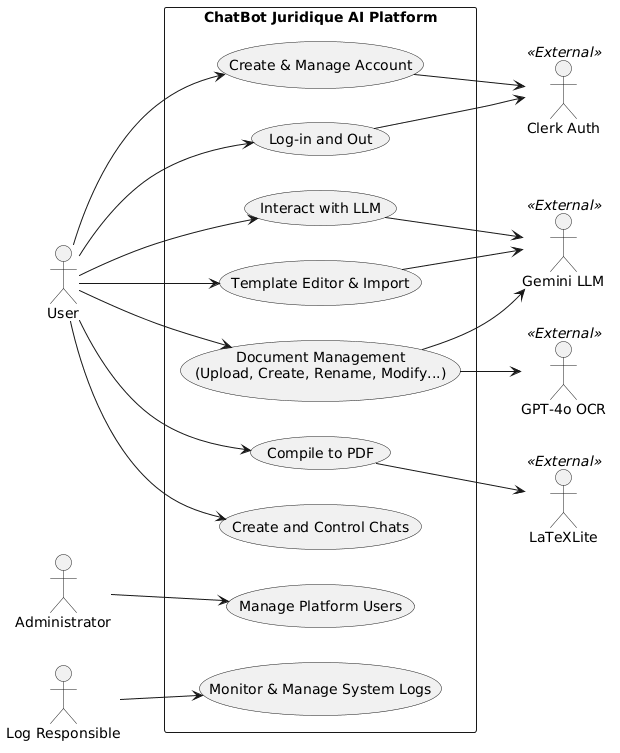
\includegraphics[width=0.75\textwidth, keepaspectratio]{Figures/use_case.png}
    }{
        \framebox[10cm]{\rule{0pt}{8cm} \textbf{Missing Image: Figures/use\_case.png}}
    }
    \caption{Global Use Case Diagram of the ChatBot Juridique AI Platform.}
    \label{fig:use_case_diagram}
\end{figure}

\newpage

\section{System Behavior (Sequence Diagrams)}
Sequence diagrams are imperative for visualizing the dynamic, temporal behavior of the system architecture. They meticulously map how internal components, backend APIs, and external services interact sequentially to execute the core functionalities of the platform.

\subsection{Chat Management and Live File Upload}
This sequence diagram comprehensively details the lifecycle of a chat session. It illustrates the workflow when a user initializes a new session, optionally uploads a live file (triggering a multimodal prompt bypass), transmits prompts to the RAG pipeline, and modifies chat metadata (e.g., renaming or pinning) via the FastAPI backend and PostgreSQL database.

\begin{figure}[H]
    \centering
    \IfFileExists{Figures/seq_chat_management.png}{
        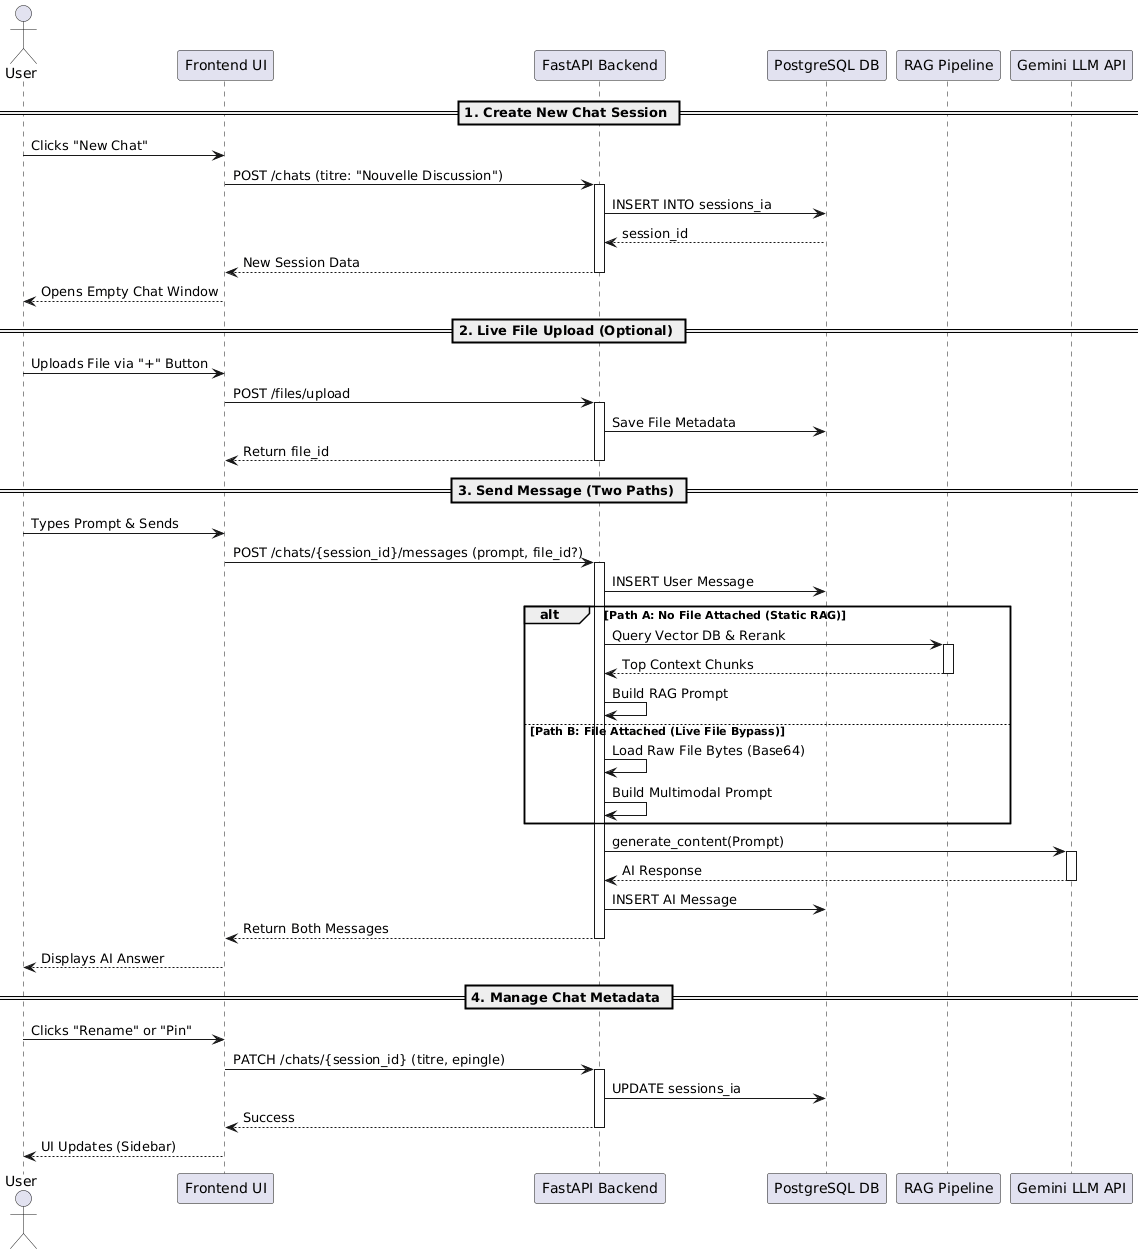
\includegraphics[width=0.9\textwidth, keepaspectratio]{Figures/seq_chat_management.png}
    }{
        \framebox[14cm]{\rule{0pt}{7cm} \textbf{Missing Image: Figures/seq\_chat\_management.png}}
    }
    \caption{Sequence Diagram illustrating Chat Session Management and Multimodal Interaction.}
    \label{fig:seq_chat_management}
\end{figure}

\newpage

\subsection{Core RAG Pipeline Execution}
This diagram maps the sophisticated query execution process when a user poses a legal question. It tracks the trajectory of the user's prompt as it is mathematically embedded, retrieved via cosine similarity in ChromaDB, rigorously reranked for maximum contextual relevance, and ultimately transmitted to the Gemini LLM to generate a factually grounded response.

\begin{figure}[H]
    \centering
    \IfFileExists{Figures/seq_rag_pipeline.png}{
        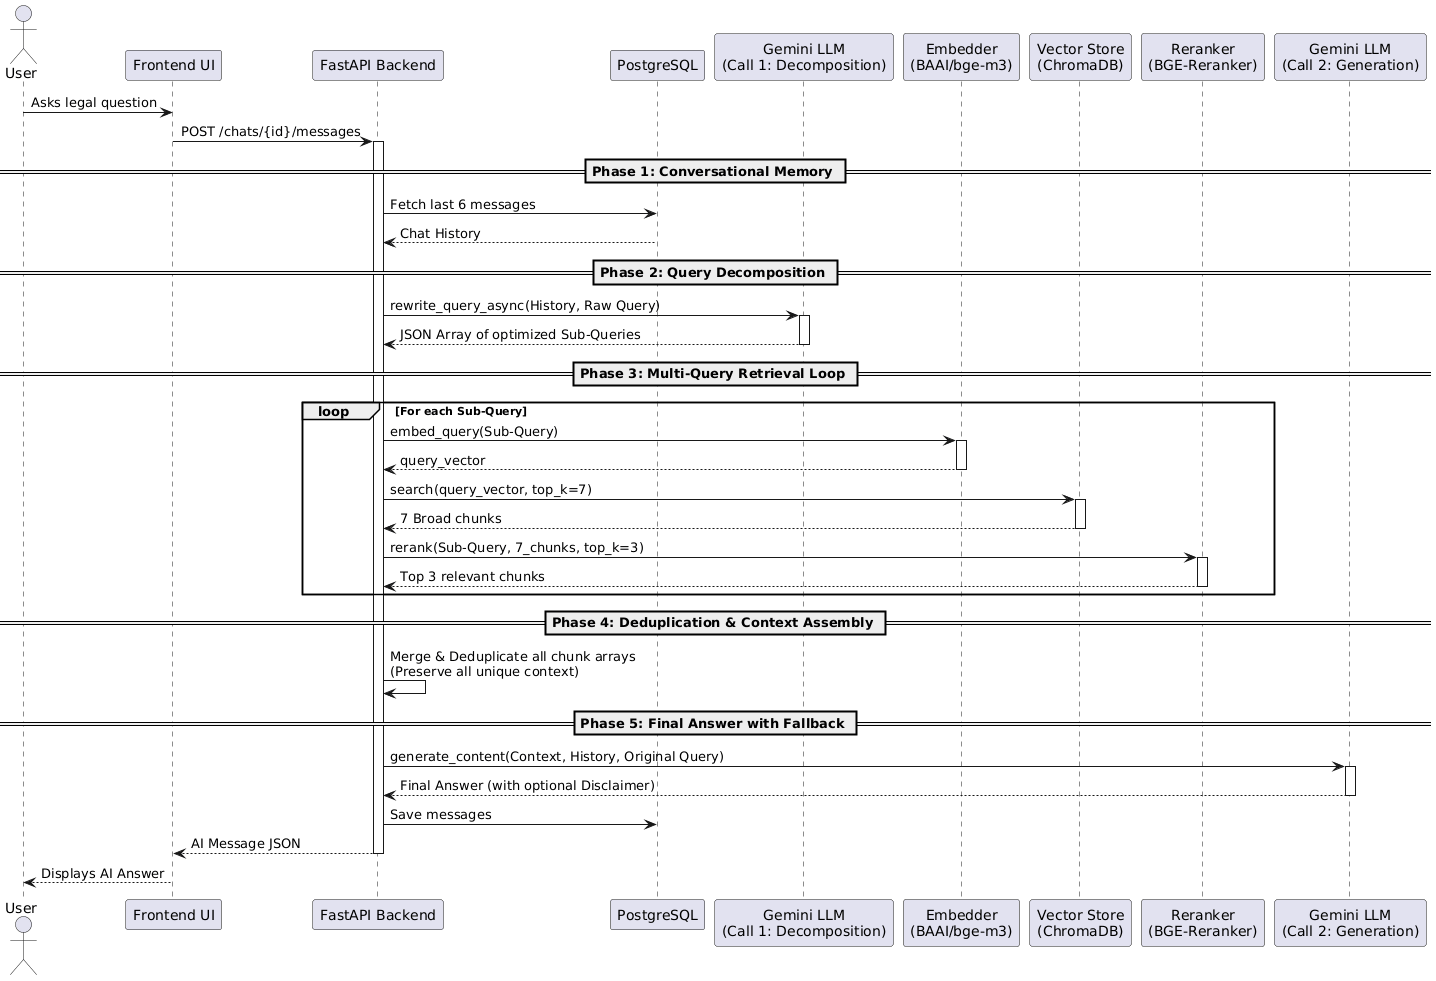
\includegraphics[width=0.9\textwidth, keepaspectratio]{Figures/seq_rag_pipeline.png}
    }{
        \framebox[14cm]{\rule{0pt}{7cm} \textbf{Missing Image: Figures/seq\_rag\_pipeline.png}}
    }
    \caption{Sequence Diagram of the Retrieval-Augmented Generation (RAG) Pipeline execution.}
    \label{fig:seq_rag}
\end{figure}

\newpage

\subsection{Document Upload and Data Ingestion}
This workflow details the highly complex offline data ingestion pipeline designed for Moroccan legal documents. It maps how raw PDFs are localized, converted into base64 images, processed by the GPT-4o Vision OCR to strip visual noise and extract semantic data, parsed by a custom XML chunker, and finally indexed into the vector database.

\begin{figure}[H]
    \centering
    \IfFileExists{Figures/seq_doc_upload.png}{
        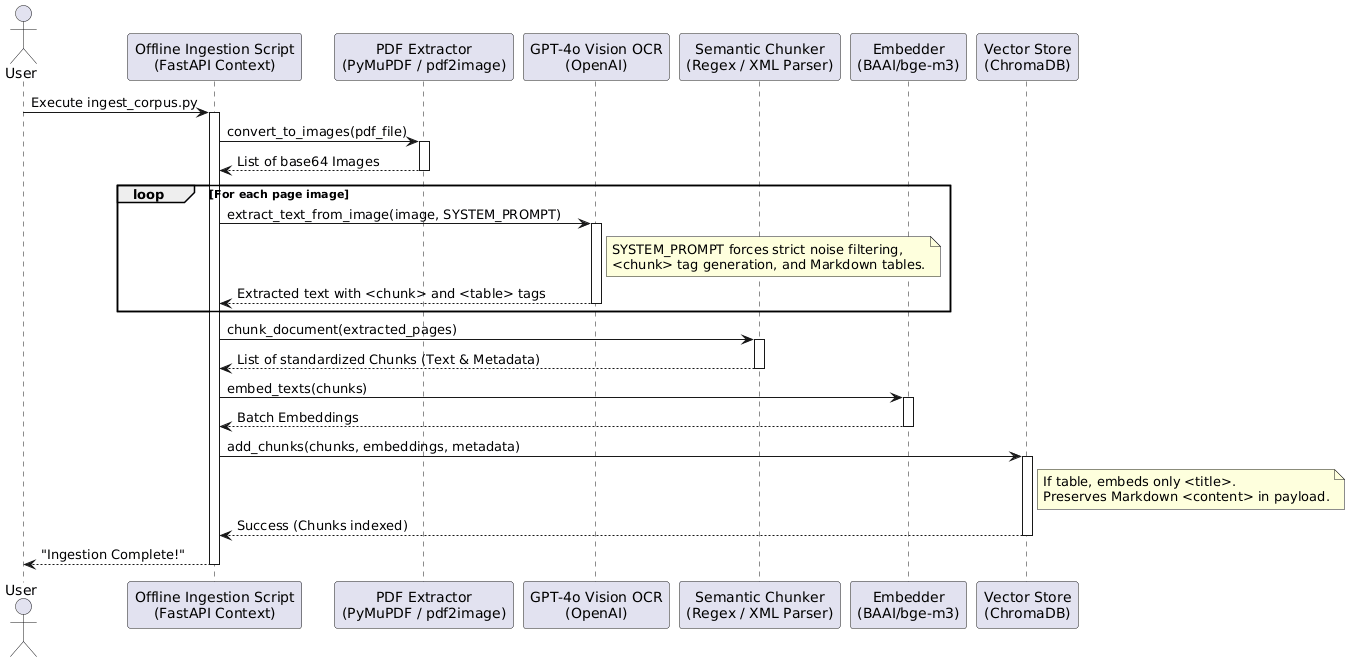
\includegraphics[width=0.9\textwidth, keepaspectratio]{Figures/seq_doc_upload.png}
    }{
        \framebox[14cm]{\rule{0pt}{7cm} \textbf{Missing Image: Figures/seq\_doc\_upload.png}}
    }
    \caption{Sequence Diagram of the Document Upload and AI-driven OCR Ingestion Process.}
    \label{fig:seq_upload}
\end{figure}

\vspace{1cm}

\subsection{AI-Assisted Document Generation}
This sequence diagram illustrates the \LaTeX\ document drafting and compilation feature. It maps how slash-commands (e.g., \texttt{/template}) trigger JSON template retrieval, which the LLM then adapts into syntactically valid \LaTeX\ code. Subsequently, it traces the dual-path compilation request—dynamically selecting between a local pdfLaTeX engine and the LaTeXLite cloud API—to render the final PDF.

\begin{figure}[H]
    \centering
    \IfFileExists{Figures/seq_doc_generation.png}{
        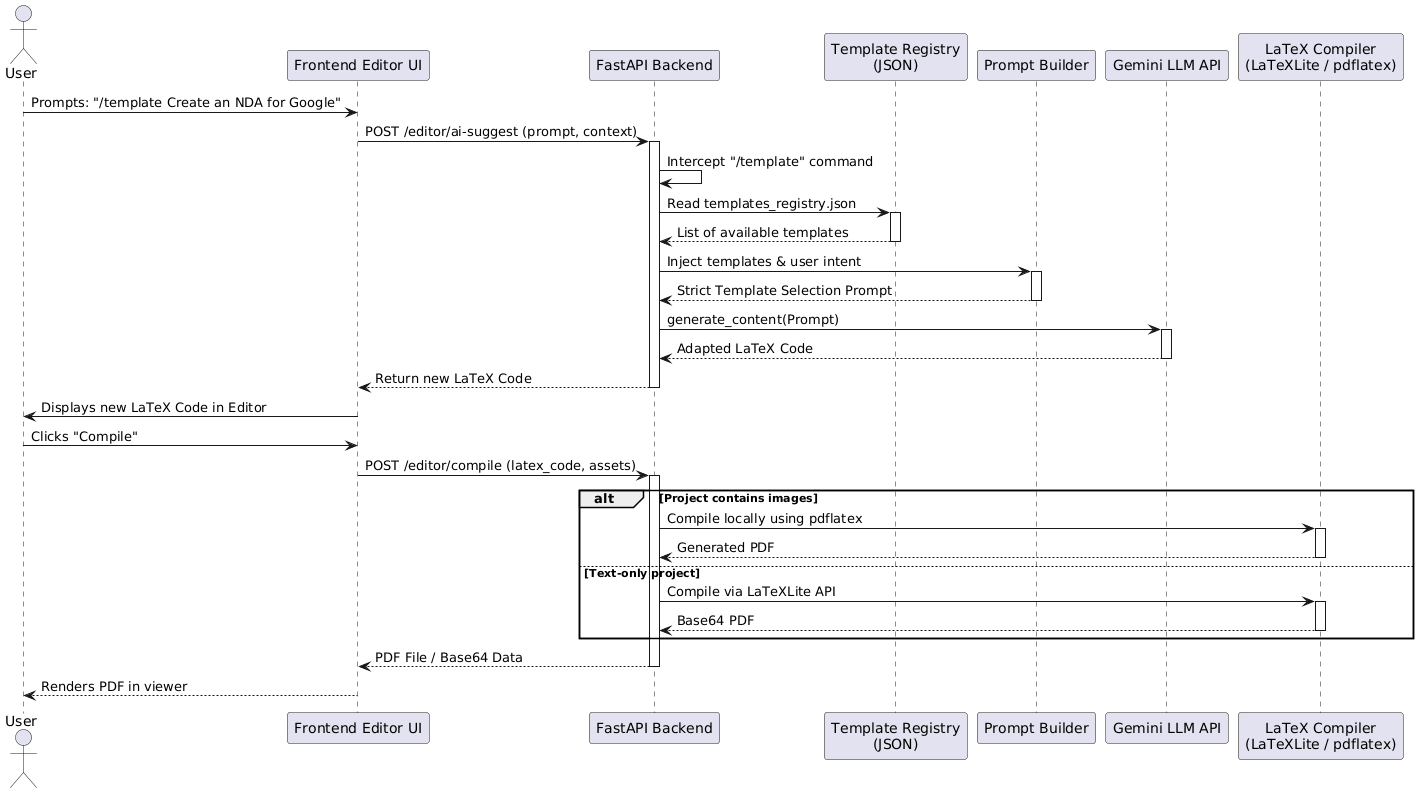
\includegraphics[width=0.9\textwidth, keepaspectratio]{Figures/seq_doc_generation.png}
    }{
        \framebox[14cm]{\rule{0pt}{7cm} \textbf{Missing Image: Figures/seq\_doc\_generation.png}}
    }
    \caption{Sequence Diagram of AI-Assisted Document Generation and Hybrid Compilation.}
    \label{fig:seq_generation}
\end{figure}

\newpage

\section{Database Architecture and Optimization}

\subsection{Class Diagram (Entity-Relationship Model)}
The Class Diagram serves as the foundational architectural blueprint for the PostgreSQL database. It illustrates the core entities—such as Users, Chat Sessions, Messages, and Documents—along with their precise attributes, primary keys, foreign keys, and relational multiplicities, ensuring a highly normalized and structurally sound data model.

\begin{figure}[H]
    \centering
    \IfFileExists{Figures/class_database.png}{
        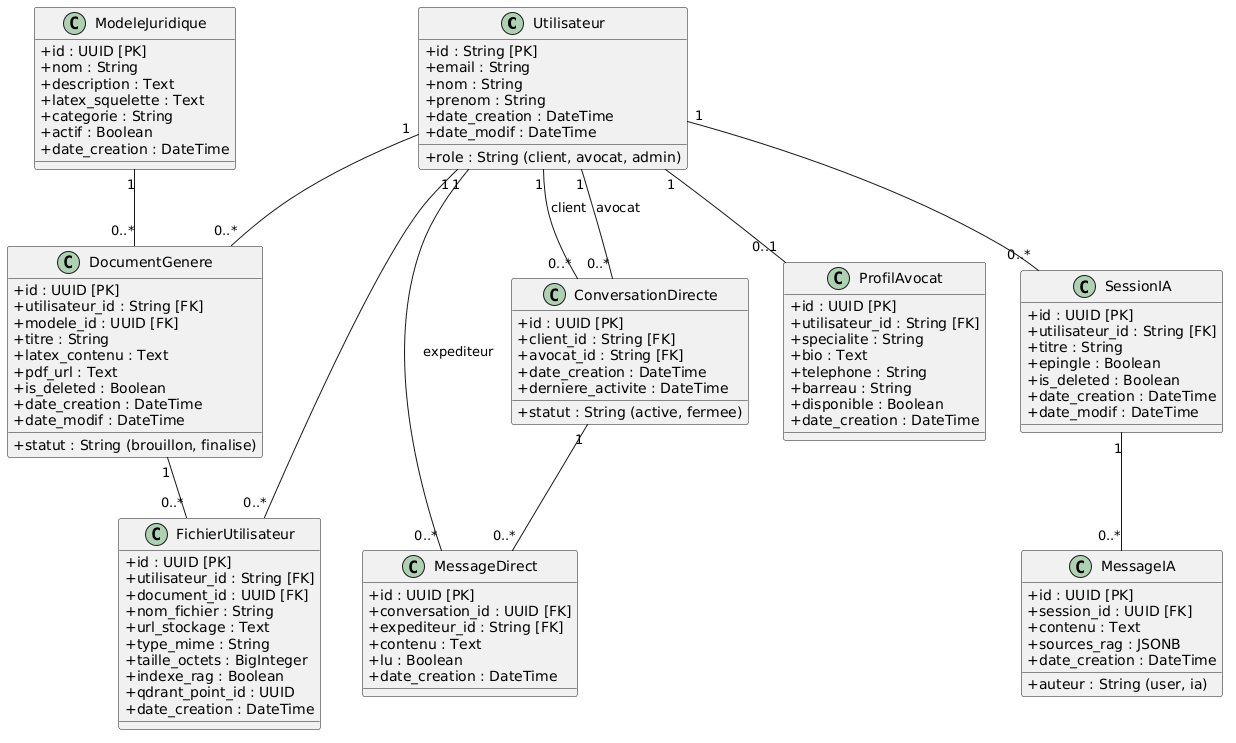
\includegraphics[width=0.9\textwidth, keepaspectratio]{Figures/class_database.png}
    }{
        \framebox[14cm]{\rule{0pt}{7cm} \textbf{Missing Image: Figures/class\_database.png}}
    }
    \caption{UML Class Diagram representing the PostgreSQL Relational Database Schema.}
    \label{fig:class_diagram}
\end{figure}

\subsection{Database Optimization Strategies}
To guarantee enterprise-grade performance, absolute data integrity, and secure tenant isolation, advanced structural optimizations were implemented directly within the PostgreSQL engine.

\begin{itemize}
    \item \textbf{Advanced Indexing Strategies:} To minimize latency on high-volume queries, several complex index structures were deployed:
    \begin{itemize}
        \item \textit{Partial \& Compound Indexes:} Deployed \texttt{idx\_sessions\_active} to index strictly active sessions while pre-sorting by \texttt{date\_modif DESC}, enabling instantaneous UI rendering.
        \item \textit{Foreign Key Indexing:} Explicitly indexed all relational foreign keys to completely eliminate full-table scans during heavy \texttt{JOIN} operations.
        \item \textit{GIN Indexing:} Applied Generalized Inverted Indexes (GIN) to RAG metadata, facilitating rapid semantic searches within JSONB payloads without requiring deserialization.
    \end{itemize}
    
    \item \textbf{PL/pgSQL Triggers \& Automation:} A custom PL/pgSQL function coupled with \texttt{BEFORE UPDATE} triggers autonomously manages all operational timestamps (e.g., dynamically setting \texttt{date\_modif} to \texttt{now()}). This ensures absolute chronological integrity and significantly reduces application-layer boilerplate logic.
    
    \item \textbf{Data Integrity \& Constraints:} Rigorous relational constraints prevent orphaned data anomalies and corrupted system states:
    \begin{itemize}
        \item \textit{Cascading Deletes (\texttt{ON DELETE CASCADE}):} All child dependencies are strictly bound to parent identifiers, ensuring pristine deletions in a single, atomic transaction.
        \item \textit{Check Constraints (\texttt{CHECK}):} Constrained vocabularies (e.g., user roles and document statuses) are strictly enforced directly on columns, rejecting malformed strings before they can corrupt the database.
    \end{itemize}
    
    \item \textbf{Aggregated Views:} A materialized SQL View (\texttt{v\_dashboard\_utilisateur}) was engineered to pre-calculate complex, heavy aggregations (such as session volumes, document counts, and RAG ingestion stats) in a single pass. This unlocks instantaneous analytics retrieval for the Dashboard API without incurring the severe performance penalties of real-time \texttt{COUNT} operations.
\end{itemize}

\section*{Conclusion}
This chapter has established a comprehensive blueprint for the platform by systematically detailing the functional, non-functional, and systemic requirements. By explicitly outlining the user interface paradigms, RAG and LLM integrations, strict performance benchmarks, and robust database optimizations, we have defined the exact technical criteria necessary for a successful implementation. These foundational specifications serve as the definitive reference guiding the software development phases discussed in subsequent chapters.

\pagebreak